% ------------------------------------------------------------------------------------------
%     前言区域
% ------------------------------------------------------------------------------------------
\documentclass[]{beamer}
\usepackage{ctex, hyperref}
\usepackage[T1]{fontenc}

% other packages
\usepackage{latexsym,amsmath,xcolor,multicol,booktabs,calligra,multirow,diagbox,array}
\usepackage{graphicx,pstricks,listings,stackengine,caption}
% ------------------------------------------------------------------------------------------
%     标题页
% ------------------------------------------------------------------------------------------
\author{潘崇林、唐溢、舒欣}
\title{基于DEA模型的中国足球协会超级联赛俱乐部效率研究}
\subtitle{系统工程小组作业}
\institute{商学院}
\date{\today}
\usepackage{GUET-Beamer}
\logo{
\includegraphics[width=0.5 cm]{Guet-logo.pdf}} % 每一页添加logo

% defs
\def\cmd#1{\texttt{\color{red}\footnotesize $\backslash$#1}}
\def\env#1{\texttt{\color{blue}\footnotesize #1}}
\definecolor{deepblue}{rgb}{0,0,0.5}
\definecolor{deepred}{rgb}{0.6,0,0}
\definecolor{deepgreen}{rgb}{0,0.5,0}
\definecolor{halfgray}{gray}{0.55}

\lstset{
    basicstyle=\ttfamily\small,
    keywordstyle=\bfseries\color{deepblue},
    emphstyle=\ttfamily\color{deepred},    % Custom highlighting style
    stringstyle=\color{deepgreen},
    numbers=left,
    numberstyle=\small\color{halfgray},
    rulesepcolor=\color{red!20!green!20!blue!20},
    frame=shadowbox,
}

\graphicspath{{./Picture/}} % 图片所在位置

% ------------------------------------------------------------------------------------------
%     正文
% ------------------------------------------------------------------------------------------
\begin{document}

\kaishu
\begin{frame}
    \titlepage
    % \begin{figure}[htpb]
    %     \vspace*{-0.3cm}
    %     \begin{center}
    %         
\includegraphics[width=0.2\linewidth]{Guet-logo.pdf}
    %     \end{center}
    % \end{figure}
\end{frame}

% \begin{frame}
%     \tableofcontents[sectionstyle=show,subsectionstyle=hide,subsubsectionstyle=hide]
% \end{frame}

\begin{frame}
    \tableofcontents[sectionstyle=show,subsectionstyle=show/shaded/hide,subsubsectionstyle=show/shaded/hide]
\end{frame}

\section{基本概念}

\subsection{DEA基本介绍}

\begin{frame}{基本概念}
    \begin{itemize}
        \item DMU(决策单元) 一个DMU就是一个将一定“输入”转换成一定“输出”的实体 
        \item T(生产可能集) 一项经济(生产)活动中必然包含x(输入)与y(产出)两项活动
        \item 规模报酬 CCR模型认为规模报酬不变,BCC模型则认为可变
    \end{itemize}
\end{frame}

\begin{frame}{生产可能集}
    \kaishu
    \begin{define}[生产可能]
        称集合 $T=\{(x, y) \mid$ 产出 $y$ 能用输入 $x$ 生产出来 $\}$ 为所有可能的生产活动构成的生产可能集。
    \end{define}
    \begin{block}{公理}
        \begin{itemize}
            \item 凸性 \ 对任意的 $(x, y) \in T$ 和 $(x', y') \in T$, 以及 $\mu \in [0,1]$ 有 $\mu(x, y)+(1-\mu)(x', y') \in T$
            \item 锥性 \ 若 $(x, y) \in T$ 及 $k \geq 0$, 则 $k(x, y)=(kx, ky) \in T$
            \item 无效性 \ 设 $(\{x\}, \{y\}) \in \{T\}$, 若 $x' \geq x$, 则 $(\{x\}', \{y\}) \in \{T\}$; 若 $y' \leq y$ 则 $(\{x\}, \{y\}') \in \{T\}$
            \item 最小性 \ 生产可能集 $\{T\}$ 是满足上述条件(1)、(2)、(3) 的所有集合的交集
        \end{itemize}
    \end{block}	
    \end{frame}

% \begin{frame}{生产函数}

% \end{frame}

\subsection{CCR模型}

\begin{frame}{相关数据}
    \resizebox{\textwidth}{!}{\begin{tabular}{|c|c|c|c|c|c|c|c|c|}
        \hline & 指标 & \begin{tabular}{l} 
        \diagbox{权数}{部门}
        \end{tabular} & 1 & 2 & & $j$ & & $n$ \\
        \hline \begin{tabular}{l} 
        投 \\
        入
        \end{tabular} & \begin{tabular}{c}
        1 \\
        2 \\
        $:$ \\
        $m$
        \end{tabular} & \begin{tabular}{c}
        $v_1$ \\
        $v_2$ \\
        $\vdots$ \\
        $v_m$
        \end{tabular} & \begin{tabular}{c}
        $x_{11}$ \\
        $x_{21}$ \\
        $:$ \\
        $x_{m 1}$
        \end{tabular} & \begin{tabular}{c}
        $x_{12}$ \\
        $x_{22}$ \\
        $:$ \\
        $x_{m 2}$
        \end{tabular} & $\ldots$ & \begin{tabular}{c}
        $x_{1 j}$ \\
        $x_{2 j}$ \\
        $:$ \\
        $x_{m j}$
        \end{tabular} & \begin{tabular}{c}
        $\cdots$ \\
        $:$
        \end{tabular} & \begin{tabular}{c}
        $x_{1 n}$ \\
        $x_{2 n}$ \\
        $:$ \\
        $x_{m n}$
        \end{tabular} \\
        \hline \begin{tabular}{l} 
        输 \\
        出
        \end{tabular} & \begin{tabular}{l}
        1 \\
        2 \\
        $:$ \\
        $q$
        \end{tabular} & \begin{tabular}{c}
        $u_1$ \\
        $u_2$ \\
        $:$ \\
        $u_p$
        \end{tabular} & \begin{tabular}{c}
        $y_{11}$ \\
        $y_{21}$ \\
        $\vdots$ \\
        $y_{p 1}$
        \end{tabular} & \begin{tabular}{c}
        $y_{12}$ \\
        $y_{22}$ \\
        $:$ \\
        $y_{p 2}$
        \end{tabular} & $\ldots$ & \begin{tabular}{c}
        $y_{1 j}$ \\
        $y_{2 j}$ \\
        $\vdots$ \\
        $y_{p j}$
        \end{tabular} & \begin{tabular}{c}
        $\cdots$ \\
        $:$
        \end{tabular} & \begin{tabular}{c}
        $y_{1 n}$ \\
        $y_{2 n}$ \\
        $\vdots$ \\
        $y_{p n}$
        \end{tabular} \\
        \hline
        \end{tabular}}
    
\end{frame}

\begin{frame}{技术效率}
技术效率指的是一个生产单元的生产过程达到本行业技术水平的程度。
第$k$个决策单元相应的效率评价指数:
$$
h_k=\frac{u_1 y_{1 k}+u_2 y_{2 k}+\cdots+u_q y_{q k}}{v_1 x_{1 k}+v_2 x_{2 k}+\cdots+v_m x_{m j}}=\frac{\displaystyle \sum_{r=1}^q u_r y_{r k}}{\displaystyle \sum_{i=1}^m v_i x_{i k}}
$$
\end{frame}

\begin{frame}{基本模型}
    \begin{align*}
        \max & \frac{\displaystyle \sum_{r=1}^q u_r y_{r k}}{\displaystyle \sum_{i=1}^m v_i x_{i k}} \\
        \text { s.t. } & \frac{\displaystyle \sum_{r=1}^q u_r y_{r k}}{\displaystyle \sum_{i=1}^m v_i x_{i k}} \leq 1 \\
        & v \geq 0 ; u \geq 0 \\
        & i=1,2, \cdots, m ; r=1,2, \cdots, q ; j=1,2, \cdots, n
    \end{align*}

\end{frame}

\begin{frame}{线性规划形式}
    \begin{align*}
        \max & \sum_{r=1}^q \mu_r y_{r k} \\
        \text { s.t. } & \sum_{r=1}^q \mu_r y_{r j}-\sum_{i=1}^m \nu_i x_{i j} \leq 0 \\
        & \sum_{i=1}^m \nu_i x_{i k}=1 \\
        & \mu \geq 0 ; \nu \geq 0 \\
        & i=1,2, \cdots, m ; r=1,2, \cdots, q ; j=1,2, \cdots, n
    \end{align*}
\end{frame}

% \begin{frame}{对偶变换}
%     \centering
%     \begin{tabular}{cccccc} 
%         & $y_{11}$ & $y_{12}$ & $\cdots$ & $y_{1 n}$ & 0 \\
%         $a_{r j}$ & $y_{21}$ & $y_{22}$ & $\cdots$ & $y_{2 n}$ & 0 \\
%         & $\vdots$ & $\vdots$ & & $\vdots$ & $\vdots$ \\
%         & $y_{p 1}$ & $y_{p 2}$ & $\cdots$ & $y_{p n}$ & 0 \\
%         \hdashline & $-x_{11}$ & $-x_{12}$ & $\cdots$ & $-x_{1 n}$ & $x_{1 j_0}$ \\
%         $a_{i j}$ & $-x_{21}$ & $-x_{22}$ & $\cdots$ & $-x_{2 n}$ & $x_{2 j_0}$ \\
%         & $\vdots$ & $\vdots$ & & $\vdots$ & $\vdots$ \\
%         & $-x_{m 1}$ & $-x_{m 2}$ & $\cdots$ & $-x_{m n}$ & $x_{m j_0}$ \\
%         \hdashline
%         \\
%         $b_j$ & 0 & 0 & $\cdots$ & 0 & 1
%     \end{tabular}
% \end{frame}

\begin{frame}{对偶形式}
    \vskip -0.5cm
    \begin{align*}
        & \min \theta \\
        \text { s.t. } & \sum_{j=1}^n \lambda_j x_{i j} \leq \theta x_{i k} \\
        & \sum_{j=1}^n \lambda_j y_{r j} \geq y_{r k} \\
        & \lambda_{j} \geq 0 \\
        & i=1,2, \cdots, m ; r=1,2, \cdots, q ; j=1,2, \cdots, n \\
    \end{align*}
\vskip -0.5cm    
$\lambda$ 表示 DMU 的线性组合系数, $k$ 表示待评价的 DMU,参数 $\theta^*$ 即为效率值,其范围在 0 到 1 之间。
% 该模型的含义相当于使用加权方法构造一个不存在的 DMU,其投入不大于待评价的 DMU,产出不小于待评价的 DMU,即 $ x=\sum_{j=1}^n \lambda_j x_{i j} , y=\sum_{j=1}^n \lambda_j y_{r j}$
\end{frame}

\begin{frame}{矩阵形式}
    \vspace*{-0.5cm}
    \begin{align*}
        & \min 0 \cdot \lambda_1+0 \cdot \lambda_2+\cdots+0 \cdot \lambda_n+1 \cdot \theta \\
        \text { s.t. } & \left[\begin{array}{ccccc}
        x_{11} & x_{12} & \cdots & x_{1 n} & -x_{1 k} \\
        x_{21} & x_{22} & \cdots & x_{2 n} & -x_{2 k} \\
        \vdots & \vdots & \cdots & \vdots & \vdots \\
        x_{m 1} & x_{m 2} & \cdots & x_{m n} & -x_{m k}
        \end{array}\right]\left[\begin{array}{c}
        \lambda_1 \\
        \lambda_2 \\
        \vdots \\
        \lambda_n \\
        \theta
        \end{array}\right] \leq\left[\begin{array}{c}
        0 \\
        0 \\
        \vdots \\
        0
        \end{array}\right] \\
        & {\left[\begin{array}{ccccc}
        -y_{11} & -y_{12} & \cdots & -y_{1 n} & 0 \\
        -y_{21} & -y_{22} & \cdots & -y_{2 n} & 0 \\
        \vdots & \vdots & \cdots & \vdots & \vdots \\
        -y_{q 1} & -y_{q 2} & \cdots & -y_{q n} & 0
        \end{array}\right]\left[\begin{array}{c}
        \lambda_1 \\
        \lambda_2 \\
        \vdots \\
        \lambda_n \\
        \theta
        \end{array}\right] 
        \leq\left[\begin{array}{c}
        -y_{1 k} \\
        -y_{2 k} \\
        \vdots \\
        -y_{q k}
        \end{array}\right]} \\
        & \lambda_j \geq 0 \\
        & i=1,2, \cdots, m ; r=1,2, \cdots, q ; j=1,2, \cdots, n \\
        &
    \end{align*}
\end{frame}

\begin{frame}{投入导向与产出导向}
    \begin{itemize}
        \item 投入导向 假设投入是固定的条件下求产出最大
        \item 产出导向 假设产出是固定的条件下求投入最小
        \item 显然 上面介绍的模型是投入导向
    \end{itemize}    
\end{frame}

\subsection{投入导向BCC模型}

\begin{frame}{对偶形式}
    \begin{align*}
        & \min  \theta \\
        \text { s.t. } & \sum_{j=1}^n \lambda_j x_{i j} \leq \theta x_{i j} \\
        & \sum_{j=1}^n \lambda_j y_{r j} \geq y_{r j} \\
        & \sum_{j=1}^n \lambda_j=1 \\
        & \lambda \geq 0 \\
        & i=1,2, \cdots, m ; r=1,2, \cdots, q ; j=1,2, \cdots, n
    \end{align*}
\end{frame}

\begin{frame}{标准形式}
    \begin{align*}
        & \min  \theta \\
        \text { s.t. } & \sum_{j=1}^n \lambda_j x_{i j} +\ s^{-}\ = \theta x_{i k} \\
        & \sum_{j=1}^n \lambda_j y_{r j} \ - s^{+}\ = y_{r k} \\
        & \sum_{j=1}^n \lambda_j=1 \\
        & \lambda \geq 0 \\
        & i=1,2, \cdots, m ; r=1,2, \cdots, q ; j=1,2, \cdots, n
    \end{align*}
\end{frame}

\begin{frame}{DEA有效性}
    $s^{-} 、 s^{+}$是松弛变量 设 CCR 与 $\mathrm{BCC}$ 模型的最优解分别为 $\lambda^* 、 s^{*-} 、 s^{*+} 、 \theta^*$, 则可对决策单元进行有效性检验. 值得注意的是, DEA 模型的有效性是 “\textcolor{red}{相对}” 有效性
    \begin{block}{有效性}
        \begin{itemize}
            \item 若 $\theta^*<1$, 决策单元为 “非有效”
            \item 若 $\theta^*=1 、 s^{*-} \neq 0 、 s^{*+} \neq 0$, 决策单元为 “弱有效”
            \item 若 $\theta^*=1 、 s^{*-}=0 、 s^{*+}=0$, 决策单元为 “有效”
        \end{itemize}    
    \end{block}    
\end{frame}

% \begin{frame}{实际意义}
%     \begin{itemize}
%         \item 综合效率(e) 
%         \item 技术效率(te)
%         \item 规模效率(se)
%         \  $lambda_{j}$ \ 
%         \item 规模报酬(rs) 
%         \ 单位产出与投入比例比随这规模变化.递增、递减、不变
%         \item 投入冗余(r) 
%         \ 
%         \item 冗余度($\alpha$) 
%         投入冗余值与投入的比值
%     \end{itemize}    
% \end{frame}

\begin{frame}{实际意义}
    \begin{tabular}{ccc}
        \toprule
        参数名称 & 符号 & 含义\\
        \midrule
        综合效率 & $e$ & $\theta^* \ e = te \times se$\\
        技术效率 & $te$ & 单独考虑技术效率,CCR则相反\\
        规模效率 & $se$ & 规模效率表示为 $\lambda_j$\\
        规模报酬 & $rs$ & 单位产出与投入比例比随规模变化,可以是\\
        & &递增、递减或不变\\
        & &$\sum_{j=1}^{n}{\lambda_j} \ ? \ 1 $\\
        & &BCC模型可以同时评估单位的效率和规模报酬\\
        投入冗余 & $\gamma$ & 也可以表示为 $s^{+}$\\
        冗余度 & $\alpha$ & 投入冗余值与投入的比值\\
        \bottomrule
    \end{tabular}
\end{frame}

\section{实际应用}

\subsection{基本介绍}

\begin{frame}{案例简介}
    基于 2015-2017 赛季中国足球协会超级联赛 (以下简称 “中超”) 俱乐部的面板数据, 从“投入产出” 角度建立俱乐部效率评价体系, 运用数据包络分析 (DEA)方法对中超俱乐部效率进行测度, 并通过效率优化解决其投入冗余问题\\
    决策单元为中超的所有俱乐部, 2015-2017 赛季中超参赛球队数目固定为 16 支, 这也符合 DEA 模型对于决策单元与投入产出指标之间数量上的要求, 即决策单元数量应多于投入与产出指标数量之和的 2 倍
\end{frame}

\begin{frame}{中超俱乐部评价体系}
    \begin{table}
        % \caption{中超俱乐部评价体系}
        \begin{tabular}{cccc}
            \toprule
            指标属性 & 变量 & 含义 & 评价目的 \\
            \midrule
            投人 & $x_1$ & 球员身价 & 人工成本 \\
            \midrule
            产出 & $y_1$ & 积分 & 成绩 \\
            & $y_2$ & 胜场 & 成绩 \\
            & $y_3$ & 进球 & 成绩 \\
            \bottomrule
        \end{tabular}
    \end{table}
    \begin{itemize}
        \item 求解工具 MATLAB、DEAP 2.1
    \end{itemize}
\end{frame}


\begin{frame}{中超俱乐部效率测度}
    \begin{table}
        % \centering
        % \caption{中超俱乐部效率测度数据}
        \vspace*{-\baselineskip}\resizebox{\textwidth}{!}{\begin{tabular}{cccccccccccccc}
            \toprule
            \multirow{2}{*}{俱乐部} & \multicolumn{4}{c}{2015 赛季} & \multicolumn{4}{c}{2016 赛季} & \multicolumn{4}{c}{2017 赛季} \\
            \cmidrule(lr){2-5} \cmidrule(lr){6-9} \cmidrule(lr){10-13}
            & 身价 & 积分 & 胜场 & 进球 & 身价 & 积分 & 胜场 & 进球 & 身价 & 积分 & 胜场 & 进球 \\
            \midrule
            广州恒大 & 4570 & 67 & 19 & 71 & 4645 & 64 & 19 & 62 & 4670 & 64 & 20 & 69 \\
            上海上港 & 1703 & 65 & 19 & 63 & 3648 & 52 & 14 & 56 & 7580 & 58 & 17 & 72 \\
            山东鲁能 & 2580 & 59 & 18 & 66 & 3163 & 34 & 9 & 38 & 2553 & 49 & 13 & 49 \\
            北京国安 & 1725 & 56 & 16 & 46 & 2128 & 43 & 11 & 34 & 2578 & 40 & 11 & 42 \\
            河南建业 & 500 & 46 & 12 & 35 & 628 & 35 & 10 & 26 & 730 & 30 & 7 & 34 \\
            上海申花 & 2163 & 42 & 12 & 42 & 2965 & 48 & 12 & 46 & 2670 & 35 & 9 & 52 \\
            石家庄永昌 & 1075 & 39 & 8 & 34 & 550 & 30 & 7 & 28 & - & - & - & - \\
            重庆力印 & 788 & 35 & 9 & 37 & 1050 & 37 & 9 & 43 & 835 & 36 & 9 & 37 \\
            江苏苏宁 & 1128 & 35 & 9 & 39 & 4503 & 57 & 17 & 53 & 4385 & 32 & 7 & 40 \\
            长春亚泰 & 1038 & 35 & 8 & 39 & 708 & 35 & 10 & 30 & 1770 & 44 & 12 & 46 \\
            杭州绿城 & 510 & 33 & 8 & 27 & 480 & 32 & 8 & 28 & - & - & - & - \\
            辽宁开新 & 853 & 31 & 7 & 30 & 720 & 36 & 9 & 38 & 710 & 18 & 4 & 30 \\
            天津泰达 & 1565 & 31 & 7 & 39 & 1258 & 36 & 9 & 38 & 2920 & 31 & 8 & 30 \\
            广州富力 & 1143 & 31 & 8 & 35 & 1265 & 40 & 11 & 47 & 1385 & 52 & 15 & 59 \\
            贵州茅台 & 1103 & 29 & 7 & 39 & - & - & - & - & - & - & - & - \\
            上海申鑫 & 385 & 17 & 4 & 30 & - & - & - & - & - & - & - & - \\
            河北华夏 & - & - & - & - & 2500 & 40 & 11 & 34 & 2218 & 52 & 15 & 55 \\
            延边富德 & - & - & - & - & 490 & 37 & 10 & 39 & 533 & 22 & 5 & 32 \\
            天津权健 & - & - & - & - & - & - & - & - & 3188 & 54 & 15 & 46 \\
            贵州智诚 & - & - & - & - & - & - & - & - & 1098 & 42 & 12 & 39 \\
            \bottomrule
        \end{tabular}}
    \end{table}
\end{frame}

% \begin{frame}{求解界面}
%     \begin{columns}
%     \begin{column}{0.5\textwidth}
%         \centering
%         % \caption{MATLAB求解}
%         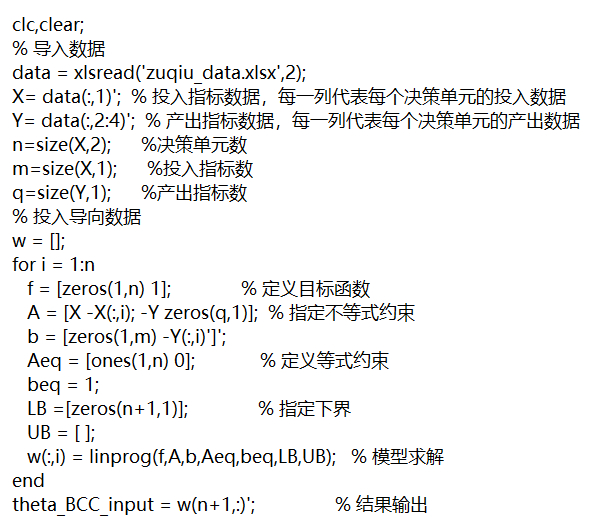
\includegraphics[width=1\linewidth]{MATLAB.jpg}
%     \end{column}
%     \begin{column}{0.5\textwidth}
%         \centering
%         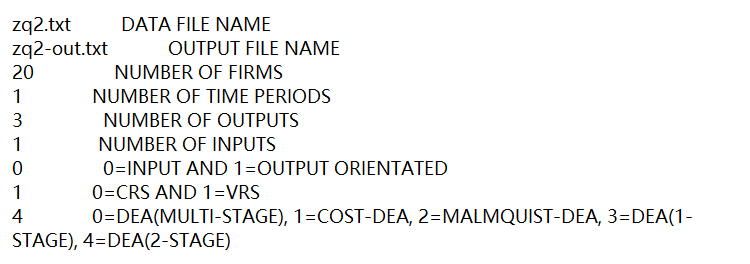
\includegraphics[width=1\linewidth]{DEAP.jpg}
%         % \caption{{DEAP\ 2.1求解}}
%     \end{column}
%     \end{columns}
% \end{frame}

\begin{frame}{指标数据处理}
    \begin{itemize}
        \item 替换指标
        \item 无量纲化处理 \ 功效系数法等
        \item \textcolor{red}{赋一个极小值} \ 如0.01、0.001等
    \end{itemize}
    \begin{block}{不变有效性}
        \begin{itemize}
            \item 推论(1) 各决策单元的同一指标数据同时扩大或缩小正的若干倍, 其 $\mathrm{DEA}$ 有效性 $\left(\mathrm{BC}^2\right)$ 不变;
            \item 推论(2) 各决策单元的同一指标数据同时加上相同的正数或适当减去相同的正数使得变换后的数据 $\left(\overline{\boldsymbol{x}}_j, \overline{\boldsymbol{y}}_j\right)>0$ 时, 其 DEA 有效性 $\left(\mathrm{BC}^2\right)$ 不变.
        \end{itemize}
    \end{block}
    上述方法处理的依据是来自DEA数据各决策单元同一指标经平移、放缩不改变其DEA有效性,但\textcolor{red}{其具体效率值可能改变}
\end{frame}

\begin{frame}{软件求解}
    \begin{columns}
        \begin{column}{0.5\textwidth}
            \begin{figure}
                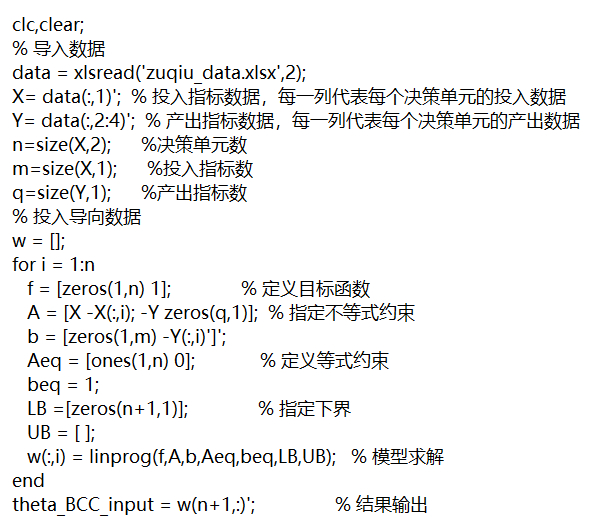
\includegraphics[width=1\linewidth]{MATLAB.jpg}
                \caption*{MATLAB求解}
            \end{figure}
        \end{column}
        \begin{column}{0.5\textwidth}
            \begin{figure}
                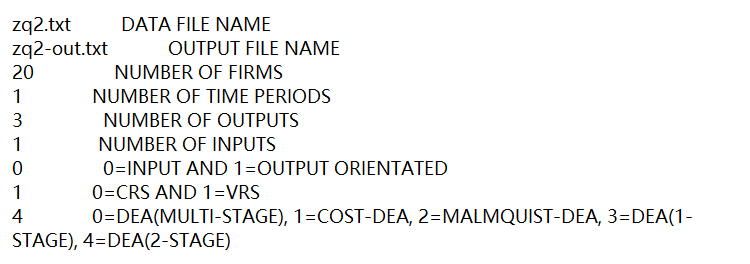
\includegraphics[width=1\linewidth]{DEAP.jpg}
                \caption*{DEAP\ 2.1求解}
            \end{figure}
        \end{column}
    \end{columns}
\end{frame}

\subsection{中超俱乐部效率评价}

\begin{frame}{效率及规模收益}
    \resizebox{\textwidth}{!}{
        \begin{tabular}{ccccccccccccc}
            \toprule
            \multirow{3}{*}{俱乐部} & \multicolumn{4}{c}{2015 赛季} & \multicolumn{4}{c}{2016 赛季} & \multicolumn{4}{c}{2017 赛季} \\
            \cmidrule(lr){2-5} \cmidrule(lr){6-9} \cmidrule(lr){10-13}
            % & 身价 & 积分 & 胜场 & 进球 & 身价 & 积分 & 胜场 & 进球 & 身价 & 积分 & 胜场 & 进球 \\
            & e & te & se & rs & e & te & se & rs & e & te & se & rs \\
            \midrule
            广州恒大 & 0.214 & 1.000 & 0.214 & drs & 0.200 & 1.000 & 0.200 & drs & 0.393 & 1.000 & 0.393 & drs \\
            上海上港 & 0.518 & 1.000 & 0.518 & drs & 0.193 & 0.903 & 0.214 & drs & 0.21 & 1.000 & 0.21 & rs \\
            山东鲁能 & 0.353 & 1.000 & 0.353 & drs & 0.151 & 0.155 & 0.976 & irs & 0.47 & 0.502 & 0.936 & drs \\
            北京国安 & 0.386 & 0.688 & 0.561 & drs & 0.268 & 0.664 & 0.403 & drs & 0.394 & 0.394 & 1.000 & crs \\
            河南建业 & 1.000 & 1.000 & 1.000 & crs & 0.780 & 0.780 & 1.000 & crs & 0.964 & 0.967 & 0.997 & irs \\
            上海申花 & 0.270 & 0.370 & 0.729 & drs & 0.214 & 0.736 & 0.291 & drs & 0.347 & 0.436 & 0.795 & drs \\
            石家庄永昌 & 0.442 & 0.444 & 0.995 & drs & 0.722 & 0.873 & 0.828 & irs & & & & \\
            重庆力帆 & 0.638 & 0.744 & 0.859 & drs & 0.515 & 0.836 & 0.616 & drs & 1.000 & 1.000 & 1.000 & crs \\
            江苏苏宁 & 0.467 & 0.596 & 0.784 & drs & 0.185 & 0.826 & 0.224 & drs & 0.173 & 0.183 & 0.944 & drs \\
            长春亚泰 & 0.506 & 0.647 & 0.782 & drs & 0.692 & 0.692 & 1.000 & crs & 0.626 & 0.627 & 0.998 & drs \\
            杭州绿城 & 0.747 & 0.879 & 0.849 & irs & 0.883 & 1.000 & 0.883 & irs & & & & \\
            辽宁开新 & 0.483 & 0.516 & 0.936 & irs & 0.663 & 0.679 & 0.976 & irs & 0.704 & 0.751 & 0.938 & irs \\
            天津泰达 & 0.331 & 0.429 & 0.771 & drs & 0.380 & 0.389 & 0.976 & irs & 0.253 & 0.26 & 0.974 & irs \\
            广州富力 & 0.413 & 0.437 & 0.945 & drs & 0.467 & 1.000 & 0.467 & drs & 1.000 & 1.000 & 1.000 & crs \\
            贵州茅台 & 0.466 & 0.609 & 0.765 & drs & & & & & & & & \\
            上海申鑫 & 1.000 & 1.000 & 1.000 & crs & & & & & & & & \\
            河北华夏 & & & & & 0.216 & 0.381 & 0.566 & drs & 0.622 & 0.624 & 0.996 & drs \\
            延边富德 & & & & & 1.000 & 1.000 & 1.000 & crs & 1.000 & 1.000 & 1.000 & crs \\
            天津权健 & & & & & & & & & 0.432 & 0.606 & 0.712 & drs \\
            贵州智诚 & & & & & & & & & 1.000 & 1.000 & 1.000 & crs \\
            均值 & 0.515 & 0.710 & 0.754 & & 0.471 & 0.745 & 0.664 & & 0.599 & 0.709 & 0.868 & \\
            \bottomrule
        \end{tabular}
    }
    % {\tiny 注: e 表示综合效率, te 表示技术效率, se 表示规模效率, rs 表示规模收益.}
\end{frame}

\begin{frame}{规模收益分析}
    \resizebox{\textwidth}{!}{
        \begin{tabular}{ccccl}
            \toprule
            \multirow{2}{*}{效率} & \multirow{2}{*}{含义} & \multicolumn{3}{c}{俱乐部} \\
            \cmidrule(lr){3-5}
            & & 2015赛季 & 2016赛季 & 2017赛季 \\
            \midrule
            $[0,0.6)$ & 无效率 & \begin{tabular}{l}
            广州恒大、上海上港、山\\
            东鲁能、北京国安、上海\\
            申花、石家庄承昌、江苏\\
            苏宁、长春亚泰、辽宁\\
            开新、天津泰达、广州富力、\\
            贵州茅台
            \end{tabular} & \begin{tabular}{l}
            广州恒大、上海上港、山\\
            东鲁能、北京国安、上海\\
            申花、重庆力帆、江苏苏\\
            宁、天津泰达、广州富力、\\
            河北华夏
            \end{tabular} & \begin{tabular}{l}
            广州恒大、上海上港、山\\
            东鲁能、北京国安、上海\\
            申花、江苏苏宁、天津泰\\
            达、天津权健
            \end{tabular} \\
            
            $[0.6,0.8)$ & 较低效率 & 重庆力帆、杭州绿城 & \begin{tabular}{l}
            河南建业、石家庄永昌、长\\
            春亚泰、辽宁开新
            \end{tabular} & \begin{tabular}{l}
            长春亚泰、辽宁开新、河北\\
            华夏
            \end{tabular} \\
            
            $[0.8,1)$ & 中等效率 & & 杭州绿㳦 & 河南建业 \\
            
            1 & 高效率 &河南建业、上海申鑫 & 延边蓄德 & \begin{tabular}{l}
            重庆力帆、广州富力、延边\\
            富德、贵州智诚
            \end{tabular} \\
            \bottomrule
        \end{tabular}
    }    
\end{frame}

\begin{frame}{中超俱乐部规模收益观察}
\begin{columns}
    \begin{column}{0.5\textwidth}
    \begin{itemize}
        \item 2015-2017赛季的48个规模收益观测值中,有\textcolor{red}{28}个为\textcolor{red}{规模收益递减},共占总体的58.3\%。
        \item 这些递减的观测值分别在各赛季中为12个、8个和8个。
        \item 这表明中超大多数俱乐部的投入都处于“\textcolor{red}{饱和型}”阶段,投入相对冗余,但由于配置不合理导致浪费现象严重,这也制约了俱乐部效率的提升。
    \end{itemize}
    \end{column}
    \begin{column}{0.5\textwidth}
    \begin{itemize}
        \item 值得注意的是,广州恒大、上海上港、上海申花和江苏苏宁这四支俱乐部在2015-2017赛季均为规模收益递减。
        \item 这一方面印证了这四支俱乐部雄厚的资金实力,但另一方面也反映了它们在资金投入的配置上仍存在一定问题。
        \item 另外,有10个观测值为规模收益递增,共占总体的20.8\%。
    \end{itemize}
    \end{column}
\end{columns}
\end{frame}

% \begin{frame}{结果分析}
%     可以看出, 2015-2017 赛季的 48 个规模收益观测值中, 有 28 个为规模收益递减,共占总体的 $58.3 \%$, 各赛季分别为 $12 、 8$ 和 8 个, 表明中超大多数俱乐部的投入都处于 “饱和型” 阶段, 俱乐部投入相对冗余, 但由于配置不合理导致浪费现象严重, 这也制约了俱乐部效率的提升. 值得注意的是, 广州恒大、上海上港、上海申花和江苏苏宁 4 支俱乐部 2015-2017 各赛季均为规模收益递减, 一方面印证了这 4 支俱乐部雄厚的资金实力; 另一方面也反映其在资金投入的配置上仍存在一定问题. 有 10 个为规模收益递增, 共占总体的 $20.8 \%$, 各赛季分别为 $2 、 5$ 和 3 个, 表明中超仅有少数俱乐部处于投入相对不足状态, 可通过进一步扩大投入规模提高俱乐部效率. 结合表 2 可以发现, 规模收益递增的俱乐部 2015-2017 各赛季积分排名均处于下游位置, 这也反映出资金投入的相对不足直接影响了俱乐部的成绩, 进而制约了俱乐部效率的提升. 值得注意的是, 辽宁开新 2015-2017 各赛季均为规模收益递增, 俱乐部长期陷入 “贫困陷莋”, 资金投入规模严重不足, 规模经济尚未形成, 最终导致在 2017 赛季降级. 有 10 个为规模收益不变, 共占总体的 $20.8 \%$, 各赛季分别为 $2 、 3$ 和 5 个, 表明中超仅有少数俱乐部处于投入配置合理状态.
% \end{frame}


% \begin{frame}{规模收益分析}
%     \begin{tabular}{ccccc}
%         \multirow{2}{*}{ 效率 } & \multirow{2}{*}{ 含义 } & \multicolumn{3}{c}{ 俱乐部 } \\
%         \hline & & 2015 赛季 & 2016 赛季 & 2017 赛季 \\
%         \hline$[0,0.6)$ & 无效率 & \begin{tabular}{l} 
%         广州恒大、上海上港、山 \\
%         东鲁能、北京国安、上海 \\
%         申花、石家庄承昌、江苏 \\
%         苏宁、长春亚泰、辽宁开 \\
%         新、天津泰达、广州富力、 \\
%         贵州茅台
%         \end{tabular} & \begin{tabular}{l} 
%         广州恒大、上海上港、山 \\
%         东鲁能、北京国安、上海 \\
%         申花、重庆力帆、江苏苏 \\
%         宁、天津泰达、广州富力、 \\
%         河北华夏
%         \end{tabular} & \begin{tabular}{l} 
%         广州恒大、上海上港、山 \\
%         东魯能、北京国安、上海 \\
%         申花、江苏苏宁、天津泰 \\
%         达、天津权健
%         \end{tabular} \\
%         \hline$[0.6,0.8)$ & 较低效率 & 重庆力㕨、杭州绿城 & \begin{tabular}{l} 
%         河南建业、石家庄永昌、长 \\
%         春亚泰、辽宁开新
%         \end{tabular} & \begin{tabular}{l} 
%         长春亚泰、辽宁开新、河北 \\
%         华夏
%         \end{tabular} \\
%         \hline$[0.8,1)$ & 中等效率 & & 杭州绿㳦 & 河南建业 \\
%         \hline 1 & 高效率 & & 延边蓄德 & \begin{tabular}{l} 
%         重庆力帆、广州富力、延边 \\
%         富德、贵州智诚
%         \end{tabular} \\
%         \hline
%         \end{tabular}
% \end{frame}

\subsection{效率优化}
\begin{frame}{效率优化}
    \resizebox{\textwidth}{!}{
        \tiny
        \begin{tabular}{ccccccc}
            \toprule
            \multirow{2}{*}{俱乐部} & \multicolumn{2}{c}{2015 赛季} & \multicolumn{2}{c}{2016 赛季} & \multicolumn{2}{c}{2017 赛季} \\
            & $r$ & $\alpha$ & $r$ & $\alpha$ & $r$ & $\alpha$ \\
            \midrule
            广州恒大 & 0.000 & $0.000$\% & 0.000 & $0.000$\% & 0.000 & $0.000$\% \\
            上海上港 & 0.000 & $0.000$\% & 355.000 & $9.731$\% & 0.000 & $0.000$\% \\
            山东鲁能 & 0.000 & $0.000$\% & 2673.909 & $84.537$\% & 1271.125 & $49.789$\% \\
            北京国安 & 537.571 & $31.164$\% & 714.667 & $33.584$\% & 1562.778 & $60.620$\% \\
            河南建业 & 0.000 & $0.000$\% & 138.000 & $21.975$\% & 24.429 & $3.346$\% \\
            上海申花 & 1362.250 & $62.980$\% & 782.222 & $26.382$\% & 1505.889 & $56.400$\% \\
            石家庄永昌 & 598.000 & $55.628$\% & 70.000 & $12.727$\% & & \\
            重庆力帆 & 202.071 & $25.644$\% & 172.500 & $16.429$\% & 0.000 & $0.000$\% \\
            江苏苏宁 & 456.143 & $40.438$\% & 781.333 & $17.351$\% & 3580.579 & $81.655$\% \\
            长春亚泰 & 366.143 & $35.274$\% & 218.000 & $30.791$\% & 660.000 & $37.288$\% \\
            杭州绿城 & 61.552 & $12.069$\% & 0.000 & $0.000$\% & & \\
            辽宁开新 & 412.483 & $48.357$\% & 230.909 & $32.071$\% & 177.000 & $24.930$\% \\
            天津泰达 & 893.143 & $57.070$\% & 768.909 & $61.122$\% & 2160.500 & $73.990$\% \\
            广州富力 & 643.000 & $56.255$\% & 0.000 & $0.000$\% & 0.000 & $0.000$\% \\
            责州茅台 & 431.143 & $39.088$\% & & & & \\
            上海申金 & 0.000 & $0.000$\% & & & & \\
            河北华夏 & & & 1548.333 & $61.933$\% & 833.000 & $37.556$\% \\
            延边富德 & & & 0.000 & $0.000$\% & 0.000 & $0.000$\% \\
            天津权健 & & & & & 1255.500 & $39.382$\% \\
            贵州智诚 & & & & & 0.000 & $0.000$\% \\
            \bottomrule
        \end{tabular}
    }
\end{frame}

\begin{frame}{中超俱乐部投入冗余情况}
\begin{columns}
    \begin{column}{0.5\textwidth}
    \begin{itemize}
        \item 2015-2017赛季中,中超俱乐部普遍存在投入冗余情况
        \item 各赛季投入冗余的俱乐部分别达到11、12、10支,占总体的68.75\%、75\%、62.5\%
        \item 这表明超过一半的俱乐部资金投入未能得到充分发挥,投入效能较低
    \end{itemize}
    \end{column}
    \begin{column}{0.5\textwidth}
    \begin{itemize}
        \item 此外,俱乐部投入冗余度也较大,排名前三的俱乐部投入冗余度均超过50\%。
        \item 结合表4可以发现,这些俱乐部的效率均落入无效率区间
        \item 这与它们高投入冗余度的结果是一致的
    \end{itemize}
    \end{column}
\end{columns}
\end{frame}

% \begin{frame}{效率优化}
%     可以看出, 2015-2017 赛季中超俱乐部普遍存在投入壳余情况, 各赛季投入宇余的俱乐部分别达到 $11 、 12 、 10$ 支, 占到总体的 $68.75 \% 、 75 \% 、 62.5 \%$. 此外, 俱乐部投入宇余度也较大, 各赛季投入冗余度排名前三俱乐部的投入冗余度均超过 $50 \%$, 这也反映出俱乐部一半以上的资金投入打了水漂, 资金的投入效能未能得到充分发挥. 结合表 4 可以发现, 这些俱乐部当赛季的俱乐部效率均落入无效率区间, 这与其高投入冗余度的结果也是相一致的.
% \end{frame}

% \section{研究现状}

% \subsection{Beamer主题分类}

% \begin{frame}
%     \begin{itemize}
%         \item 有一些 \LaTeX{} 自带的
%         \item 有一些GUET的
%         \item 本模板来源自 \newline \url{https://www.latexstudio.net/archives/4051.html}
%         \item 但是最初的 \href{http://far.tooold.cn/post/latex/beamerdlut}{\color{purple}{link}} \cite{origin}已经失效了
%         \item 整体设计参考自[Trinkle23897 / THU-Beamer-Theme](https://github.com/Trinkle23897/THU-Beamer-Theme)
%     \end{itemize}
% \end{frame}

% \section{研究内容}

% \subsection{美化主题}

% \begin{frame}{主题说明}
%     \begin{itemize}
%         \item 顶栏的小点变成一行而不是多行
%         \item 中文采用楷书
%         \item 更多该模板的功能可以参考 \url{https://www.latexstudio.net/archives/4051.html}
%         \item 下面列举出了一些Beamer的用法,部分节选自 \url{https://tuna.moe/event/2018/latex/}
%     \end{itemize}
% \end{frame}

% \subsection{如何更好地做Beamer}

% \begin{frame}{Why Beamer}
%     \begin{itemize}
%         \item \LaTeX 广泛用于学术界,期刊会议论文模板
%     \end{itemize}
%     \begin{table}[h]
%         \centering
%         \begin{tabular}{c|c}
%             Microsoft\textsuperscript{\textregistered}  Word & \LaTeX \\
%             \hline
%             文字处理工具 & 专业排版软件 \\
%             容易上手,简单直观 & 容易上手 \\
%             所见即所得 & 所见即所想,所想即所得 \\
%             高级功能不易掌握 & 进阶难,但一般用不到 \\
%             处理长文档需要丰富经验 & 和短文档处理基本无异 \\
%             花费大量时间调格式 & 无需担心格式,专心作者内容 \\
%             公式排版差强人意 & 尤其擅长公式排版 \\
%             二进制格式,兼容性差 & 文本文件,易读、稳定 \\
%             付费商业许可 & 自由免费使用 \\
%         \end{tabular}
%     \end{table}
% \end{frame}

% \begin{frame}{排版举例}
	
% 	\begin{textbox}{无编号公式}
%         \begin{equation*}
%             J(\theta) = \mathbb{E}_{\pi_\theta}[G_t] = \sum_{s\in\mathcal{S}} d^\pi (s)V^\pi(s)=\sum_{s\in\mathcal{S}} d^\pi(s)\sum_{a\in\mathcal{A}}\pi_\theta(a|s)Q^\pi(s,a)
%         \end{equation*}
%     \end{textbox}
%     \begin{textbox}{多行多列公式\footnotemark[1]}
%         % 使用 & 分隔
%         \begin{align}
%             Q_\mathrm{target}&=r+\gamma Q^\pi(s^\prime, \pi_\theta(s^\prime)+\epsilon)\\
%             \epsilon&\sim\mathrm{clip}(\mathcal{N}(0, \sigma), -c, c)\nonumber
%         \end{align}
%     \end{textbox}
%     \footnotetext[1]{如果公式中有文字出现,请用 $\backslash$mathrm\{\} 或者 $\backslash$text\{\} 包含,不然就会变成 $clip$,在公式里看起来比 $\mathrm{clip}$ 丑非常多。}
% \end{frame}


% \begin{frame}{如何使用块}
% \begin{block}{块的名称}
% 	\begin{itemize}
%         \item A
%         \item B
%     \end{itemize}
% \end{block}	
% \end{frame}

% \begin{frame}{如何使用定义、定理、引理、证明}

% \kaishu
% \begin{define}[定义名称]
% 	定义内容
% \end{define}

% \begin{lem}[引理名称]
% 	引理内容
% \end{lem}

% \begin{thm}[定理名称]
% 	定理内容(这里的定义、引理、定理分章节自动标号)
% \end{thm}

% \begin{proof}
% 	证明内容
% \end{proof}

% \end{frame}

% \begin{frame}
%     \begin{textbox}{编号多行公式}
%         % Taken from Mathmode.tex
%         \begin{multline}
%             A=\lim_{n\rightarrow\infty}\Delta x\left(a^{2}+\left(a^{2}+2a\Delta x+\left(\Delta x\right)^{2}\right)\right.\label{eq:reset}\\
%             +\left(a^{2}+2\cdot2a\Delta x+2^{2}\left(\Delta x\right)^{2}\right)\\
%             +\left(a^{2}+2\cdot3a\Delta x+3^{2}\left(\Delta x\right)^{2}\right)\\
%             +\ldots\\
%             \left.+\left(a^{2}+2\cdot(n-1)a\Delta x+(n-1)^{2}\left(\Delta x\right)^{2}\right)\right)\\
%             =\frac{1}{3}\left(b^{3}-a^{3}\right)
%         \end{multline}
%     \end{textbox}
% \end{frame}

% \begin{frame}{图形与分栏}
%     % From thuthesis user guide.
%     \begin{minipage}[c]{0.3\linewidth}
%         \psset{unit=0.8cm}
%         \begin{pspicture}(-1.75,-3)(3.25,4)
%             \psline[linewidth=0.25pt](0,0)(0,4)
%             \rput[tl]{0}(0.2,2){$\vec e_z$}
%             \rput[tr]{0}(-0.9,1.4){$\vec e$}
%             \rput[tl]{0}(2.8,-1.1){$\vec C_{ptm{ext}}$}
%             \rput[br]{0}(-0.3,2.1){$\theta$}
%             \rput{25}(0,0){%
%             \psframe[fillstyle=solid,fillcolor=lightgray,linewidth=.8pt](-0.1,-3.2)(0.1,0)}
%             \rput{25}(0,0){%
%             \psellipse[fillstyle=solid,fillcolor=yellow,linewidth=3pt](0,0)(1.5,0.5)}
%             \rput{25}(0,0){%
%             \psframe[fillstyle=solid,fillcolor=lightgray,linewidth=.8pt](-0.1,0)(0.1,3.2)}
%             \rput{25}(0,0){\psline[linecolor=red,linewidth=1.5pt]{->}(0,0)(0.,2)}
% %           \psRotation{0}(0,3.5){$\dot\phi$}
% %           \psRotation{25}(-1.2,2.6){$\dot\psi$}
%             \psline[linecolor=red,linewidth=1.25pt]{->}(0,0)(0,2)
%             \psline[linecolor=red,linewidth=1.25pt]{->}(0,0)(3,-1)
%             \psline[linecolor=red,linewidth=1.25pt]{->}(0,0)(2.85,-0.95)
%             \psarc{->}{2.1}{90}{112.5}
%             \rput[bl](.1,.01){C}
%         \end{pspicture}
%     \end{minipage}\hspace{1cm}
%     \begin{minipage}{0.5\linewidth}
%         \medskip
%         %\hspace{2cm}
%         \begin{figure}[h]
%             \centering
%             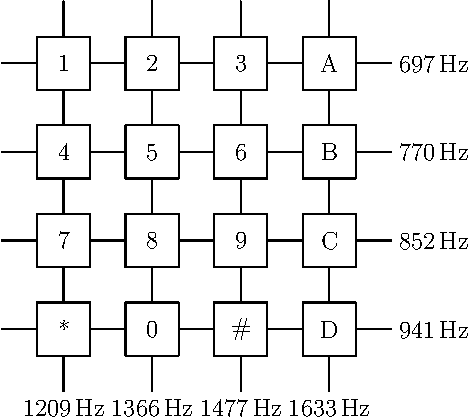
\includegraphics[height=.4\textheight]{dtmf.pdf}
%         \end{figure}
%     \end{minipage}
% \end{frame}




% \begin{frame}[fragile]{\LaTeX{} 常用命令}
%     \begin{textbox}{命令}
%     	\centering
%         \footnotesize
%         \begin{tabular}{llll}
%             \cmd{chapter} & \cmd{section} & \cmd{subsection} & \cmd{paragraph} \\
%             章 & 节 & 小节 & 带题头段落 \\\hline
%             \cmd{centering} & \cmd{emph} & \cmd{verb} & \cmd{url} \\
%             居中对齐 & 强调 & 原样输出 & 超链接 \\\hline
%             \cmd{footnote} & \cmd{item} & \cmd{caption} & \cmd{includegraphics} \\
%             脚注 & 列表条目 & 标题 & 插入图片 \\\hline
%             \cmd{label} & \cmd{cite} & \cmd{ref} \\
%             标号 & 引用参考文献 & 引用图表公式等\\\hline
%        	\end{tabular}
%     \end{textbox}
%     \begin{textbox}{环境}
%         \centering
%         \footnotesize
%         \begin{tabular}{lll}
%             \env{table} & \env{figure} & \env{equation}\\
%             表格 & 图片 & 公式 \\\hline
%             \env{itemize} & \env{enumerate} & \env{description}\\
%             无编号列表 & 编号列表 & 描述 \\\hline
%         \end{tabular}
%     \end{textbox}
% \end{frame}

% \begin{frame}[fragile]{\LaTeX{} 环境命令举例}
%     \begin{minipage}{0.5\linewidth}
% \begin{lstlisting}[language=TeX]
% \begin{itemize}
%   \item A \item B
%   \item C
%   \begin{itemize}
%     \item C-1
%   \end{itemize}
% \end{itemize}
% \end{lstlisting}
%     \end{minipage}\hspace{1cm}
%     \begin{minipage}{0.3\linewidth}
%         \begin{itemize}
%             \item A
%             \item B
%             \item C
%             \begin{itemize}
%                 \item C-1
%             \end{itemize}
%         \end{itemize}
%     \end{minipage}
%     \medskip
%     \pause
%     \begin{minipage}{0.5\linewidth}
% \begin{lstlisting}[language=TeX]
% \begin{enumerate}
%   \item 巨佬 \item 大佬
%   \item 萌新
%   \begin{itemize}
%     \item[n+e] 瑟瑟发抖
%   \end{itemize}
% \end{enumerate}
% \end{lstlisting}
%     \end{minipage}\hspace{1cm}
%     \begin{minipage}{0.3\linewidth}
%         \begin{enumerate}
%             \item 巨佬
%             \item 大佬
%             \item 萌新
%             \begin{itemize}
%                 \item[n+e] 瑟瑟发抖
%             \end{itemize}
%         \end{enumerate}
%     \end{minipage}
% \end{frame}

% \begin{frame}[fragile]{\LaTeX{} 数学公式}
%     \begin{columns}
%         \begin{column}{.55\textwidth}
% \begin{lstlisting}[language=TeX]
% $V = \frac{4}{3}\pi r^3$

% \[
%   V = \frac{4}{3}\pi r^3
% \]

% \begin{equation}
%   \label{eq:vsphere}
%   V = \frac{4}{3}\pi r^3
% \end{equation}
% \end{lstlisting}
%         \end{column}
%         \begin{column}{.4\textwidth}
%             $V = \frac{4}{3}\pi r^3$
%             \[
%                 V = \frac{4}{3}\pi r^3
%             \]
%             \begin{equation}
%                 \label{eq:vsphere}
%                 V = \frac{4}{3}\pi r^3
%             \end{equation}
%         \end{column}
%     \end{columns}
%     \begin{itemize}
%         \item 更多内容请看 \href{https://zh.wikipedia.org/wiki/Help:数学公式}{\color{purple}{这里}}
%     \end{itemize}
% \end{frame}

% \begin{frame}[fragile]
%     \begin{columns}
%         \column{.6\textwidth}
% \begin{lstlisting}[language=TeX]
%     \begin{table}[htbp]
%       \caption{编号与含义}
%       \label{tab:number}
%       \centering
%       \begin{tabular}{cl}
%         \toprule
%         编号 & 含义 \\
%         \midrule
%         1 & 4.0 \\
%         2 & 3.7 \\
%         \bottomrule
%       \end{tabular}
%     \end{table}
%     公式~(\ref{eq:vsphere}) 的
%     编号与含义请参见
%     表~\ref{tab:number}。
% \end{lstlisting}
%         \column{.4\textwidth}
%         \begin{table}[htpb]
%             \centering
%             \caption{编号与含义}
%             \label{tab:number}
%             \begin{tabular}{cl}\toprule
%                 编号 & 含义 \\\midrule
%                 1 & 4.0\\
%                 2 & 3.7\\\bottomrule
%             \end{tabular}
%         \end{table}
%         \normalsize 公式~(\ref{eq:vsphere})的编号与含义请参见表~\ref{tab:number}。
%     \end{columns}
% \end{frame}

% \begin{frame}{作图}
%     \begin{itemize}
%         \item 矢量图 eps, ps, pdf
%         \begin{itemize}
%             \item METAPOST, pstricks, pgf $\ldots$
%             \item Xfig, Dia, Visio, Inkscape $\ldots$
%             \item Matlab / Excel 等保存为 pdf
%         \end{itemize}
%         \item 标量图 png, jpg, tiff $\ldots$
%         \begin{itemize}
%             \item 提高清晰度,避免发虚
%             \item 应尽量避免使用
%         \end{itemize}
%     \end{itemize}
%     \begin{figure}[htpb]
%         \centering
%         
\includegraphics[width=0.2\linewidth]{Guet-logo.pdf}
%         \caption{这个校徽就是矢量图}
%     \end{figure}
% \end{frame}


% \section{计划进度}
% \begin{frame}
%     \begin{itemize}
%         \item 一月:完成文献调研
%         \item 二月:复现并评测各种Beamer主题美观程度
%         \item 三、四月:美化GUET Beamer主题
%         \item 五月:论文撰写
%     \end{itemize}
% \end{frame}


\section{参考文献}

\begin{frame}{参考文献}
    \nocite{*}
    \bibliography{ref.bib}
    \bibliographystyle{alpha}
    % 如果参考文献太多的话,可以像下面这样调整字体:
    % \tiny\bibliographystyle{alpha}
\end{frame}

\begin{frame}
    \begin{center}
        {\Huge\calligra Thanks!}
    \end{center}
\end{frame}

\end{document}